\documentclass[12pt,a4paper,twoside]{article}
\usepackage{polski}
\usepackage[utf8]{inputenc}
\usepackage[left=3.5cm,right=2.5cm,top=2.5cm,bottom=2.5cm]{geometry}
\usepackage{graphicx}
\usepackage{lipsum}
\usepackage{setspace}
\spacing{1.15}
\setlength{\parindent}{1.25cm}
%% ########################################################
\begin{document}
\thispagestyle{empty}
\begin{center}

\includegraphics[width=\textwidth]{img/logo_AGH.jpg}\\
{\bf{\sf WYDZIAŁ GEOLOGII, GEOFIZYKI I OCHRONY ŚRODOWISKA}}\\[5mm]
%% ======================================================
{\bf{\sf{KATEDRA GEOINFORMATYKI I INFORMATYKI STOSOWANEJ}}}\\[14mm]

{\sf{\huge Projekt dyplomowy}}\\[12mm] 
%% ======================================================
{\sf{\Large Aplikacja do zarządzania zbiorami danych\\[2mm] 
Dataset management application}}\\[40mm]
\end{center}
{\sf\begin{tabular}{ll}
	Autor: & Monika Hertel\\
	Kierunek studiów: & Inżynieria i Analiza Danych\\
	Opiekun pracy: & dr Paweł Oleksik\\
\end{tabular}}\\[10mm]
\begin{center}
{\sf Kraków, 2024}
\end{center}
%% ########################################################
\newpage
\tableofcontents
\newpage
\section*{Wstęp}
\addcontentsline{toc}{section}{Wstęp}
W czasach przeciążonych informacją, 
\newpage
%% ########################################################
\section{Zagadnienia teoretyczne}
%% ########################################################
\subsection{Problem tworzenia streszczeń}
(wspomnieć o tym żę niektóre pdf posiadają outlines i wtedy są slay)
Streszczenie w każdej pracy naukowej jest jej ważną częścią. Ma ono na celu przekazać kluczowe informacje o czytanym dokumencie, aby czytelnik mógł ocenić czy dany artykuł (jest dla niego). Automatyzacja tego procesu dąży do ułatwienia autorom tworzenia prac, poprzez skrócenie czasu, którego wymaga kreacja abstraktu. Systemy ATS (ang. \textit{Automatic Text Summarization}) są jednym z cięższych wyzwań sztucznej inteligencji, dotyczących przetwarzania języka naturalnego. Metody wytwarzania streszczeń możemy podzielić na ekstraktywane i abstrakcyjne.
\subsubsection*{Ekstraktywne a Abstrakcyjne}
Podejście ekstraktywne polega na wybraniu najważniejszych zdań z całego dokumentu. Algorytm sam w sobie nie tworzy nowych zdań, dlatego też w często jest tak że zdania nie mają sensu w takiej kolejności\par
Tworzenie streszczeń metodami abstrakcyjnymi 
\newpage
%% ########################################################
\subsection{Tworzenie aplikacji webowych}
W proces tworzenia aplikacji wchodzi wiele elementów. Wybór odpowiednich narzędzi jest jednym nich. 
%% ########################################################
\subsection{Ekstrakcja słów z plików pdf}
unicode  albo że nie wykrywa poprawnie słów, jakby da się ale nie pod kontem tworzenia streszczeń czy coś czy tagowania bo nie chcemy brać pod uwagę stopek itp
\section{Implementacja}
\subsection{Projekt systemu}
System ma na celu ułatwienie przechowywania plików zawierających informacje. Pliki, po dostarczeniu przez użytkownika, są przenoszone do dedykowanego folderu aplikacji. Sprawdzany jest typ pliku i zgodnie z nim wykonywane są inne akcje. Dla plików o rozszeżeniu pdf pobierana jest zawartość i z niej powstaje streszczenie i słowa klucze. Potem wszystkie informacje umieszczane są w bazie danych tak, aby użytkownik mógł wyszukać z użyciem aplikacji dany pliki. \par
%% ########################################################
\subsection{Struktura aplikacji}
(kiedy zaczynałam apke to robiłam ją z templatki electron+react (link) do której dokleiłam server python)
Aplikacja została zbudowana z myślą o zapewnieniu interfejsu użytkownika przy użyciu JavaScript React, serwera HTTP opartego na Flask Python, oraz bazy danych MongoDB, która jest bazą typu NoSQL. Zintegrowana całość jest uruchamiana z wykorzystaniem pakietu Electron, co umożliwia stworzenie aplikacji natywnej, zachowując przy tym funkcje przeglądarki oraz pozwalając na dostęp do zasobów systemowych.
\subsubsection*{Javascript React}
Jest to biblioteką pozwalająca na budowanie interaktywnych interfejsów użytkownika. Główną koncepcją React są komponenty, czyli samodzielne, hermetyczne jednostku interfejsu. Pozwala to na reakcje na zmiany wywołane przez użytkownika lub sam system i przy tym automatyczne aktualizowanie tych stron. React używa składni JSX (\textit{Javascript XML}), który jest rozszerzeniem składni Javascript. Integruje ona kod Javascript z deklaratywnym opisem struktury interfejsu.
\subsubsection*{Python Flask}
Na potrzeby tego projektu, mikroserwis jakim jest flask, jest wystarczający do zaprezentowania idei aplikacji. Jest on elastyczny i prosty w urzytkowaniu. Najważniejszą jego cechą, z punktu widxenia tej pracy jest fakt, że jest on biblioteką języka python. W pierwszej fazie testów używanych algorytmów, były one tworzone z pomocą tego języka. Python jest językiem często używanym w szerokim spektrum tematu jakim jest sztuczna inteligencja.\par
Obsługa serweru HTTP poprzez moduł \textit{Flask} jest dokonywana z użyciem dekoratorów. Dekoratory te definiują \textit{routes} na jakie odpowiada dana funkcja. Pisanie takiej funkcji jest ograniczone jedynie poprzez strukturę odpowiedzi zwrotnej (return function). Funkcja musi zwrócić obiekt, któy jest w stanie przejść przez komunikat HTTP (nwm jak to nazwać inaczej, musi się dać przenieść). Tutaj serwer jest traktowany jako narzędzie umożliwiające kożystanie z bibliotek języka python. W innych sytuacjach, kiedy tworzenie aplikacji jest robione całkowicie w pythonie, możliwe jest tworzenie templatek do których dodawane są wartości z funkcji. (lol dokumentacja)
\begin{figure}[h!]
\centering
  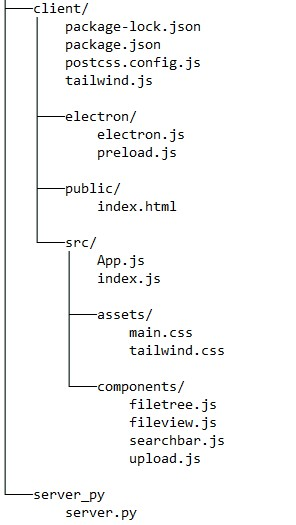
\includegraphics{img/file_structure.jpg}
  \caption{Uogólniona struktura projektu}
\end{figure}
\newpage
%% ########################################################
\subsection{Architektura systemu} %omg electron+react+flask
\subsubsection*{Baza danych}
\newpage
%% ########################################################
\subsection{Scenariusze wykorzystania aplikacji}
Aplikacja przyjmuje pliki o rozszerzeniu pdf, txt i csv. Zachowanie systemu przy dodaniu pierwszych dwóch rodzajów plików, zachowuje się podobnie. Skupmy się na plikach pdf.
\begin{enumerate}
	\item Gdy użytkownik wybierze plik, aplikacja przesyła ścieżkę pliku do serwera,
	\item System wyciąga z pliku cały tekst z pomocą biblioteki języka Python \textit{PdfMiner},
	\item Z zawartości zostają wyciągnięte słowa klucze. Tworzenie tzw. tagów odbywa się z pomocą biblioteki \textit{yake} oraz funkcji \textit{KeywordExtractor()}. Funkcja ta przyjmuje variables dotyczące języka danego tekstu, maksymalną ilość słów w tagu, ponieważ możemy ustawić ich więcej niż 1, deduplication treshold który definiuje szansę na powtóżenie się słów w różnych tagach (im bliżej 0 tym mniejsze prawdopodobieństwo), oraz oczekiwaną liczbę słów kluczowych. 
	\item w tym samym czasie z pomocą biblioteki \textit{sumy} oraz funkcji \textit{TextRankSummarizer}, jest tworzone streszczenie metodą ekstraktywną, polegającą na (opis TextRank)\
	\item jeżeli plik pdf posiada outlines to metoda \textit{.get\_outlines()} ekstraktuje je i z wyniku możemy wyciągnąć tytuł dokumentu i nadać plikowi taką nazwę. a jeżeli ich nie ma to tytułem pliku zostaje pierwsze słowo kluczowe
	\item ostatecznie wszystkie informacje są zbierane i przesyłane do bazy danych w poniższej formie
\end{enumerate}
\begin{figure}[h]
\centering
  \includegraphics[width=\textwidth]{img/file\_add\_pl.png}
  \caption{Schemat sekwencyjny dodawania pliku}
\end{figure}
\subsubsection*{Wyszukiwanie i wyświetlanie plików}
Użytkownik ma możliwość wysukiwania plików po słowach kluczach lub tytule pliku. Tutaj przydatne jest użycie API generującego synonimy dla wyszukiwanego słowa. System zachowuje się w poniżej opisany sposób.
\begin{enumerate}
	\item aplikacja przesyła komunikat ze słowem wyszukiwanym tzn POST /search\_bar,
	\item serwer używając API synonimów pobiera 5 najbliższych słów do słowa szukanego przypisując im ranking,
	\item serwer przesyła osobne komunikaty do tabeli \textit{file\_properties} w naszej bazie danych, zawierające osobno słowo klucz oraz synonimy
	\item baza zwraca komunikaty ze znalezionymi dokumentami oraz szukanym słowem, na co server przypisuje im wagi
	\item serwer zwraca listę plików użytkownikowi, posortowane zgodnie z rankingiem
\end{enumerate}
\begin{figure}[h]
\centering
  \includegraphics[width=\textwidth]{img/file\_search.png}
  \caption{Schemat sekwencyjny wyszukiwania pliku}
\end{figure}
\newpage
%% ########################################################
\subsection{Testy funkcjonalne}
%% ########################################################
\subsection{TEMP Idealna aplikacja}
Dla każdego pliku aplikacja ma opcje. 
%% ########################################################
\section{Możliwości rozwoju i wykorzystania aplikacji}
%% ########################################################
\subsection{Przetwarzanie obrazów}
%% ########################################################
\subsection{Rozbudowanie funkcjonalności dla plików bazodanowych}
%% ########################################################
\subsection{Przejście na wersje web}
%% ########################################################
\section*{Podsumowanie i wnioski}
\addcontentsline{toc}{section}{Podsumowanie i wnioski}
W sumie to nie wiem co jest celem tej pracy ani co mam podsumować, 
%% ########################################################
\listoffigures
\addcontentsline{toc}{section}{Spis Rysunków}
\end{document}